Let $m,n \ge 3$ be integers.
Nemo is given an $m \times n$ grid of unit squares with one chip on every unit square initially.
They can repeatedly carry out the following operation:
first, they pick any three distinct collinear unit squares and
then they move one chip from each of the outer two squares onto the middle square.
They may only do this operation if the outer two squares are not empty,
but the middle square is allowed to be empty. 
As a function of $(m,n)$, either determine the maximum number of operations Nemo can make
before they cannot continue anymore, or prove that they can carry out an arbitrarily large number of operations.

\begin{center}
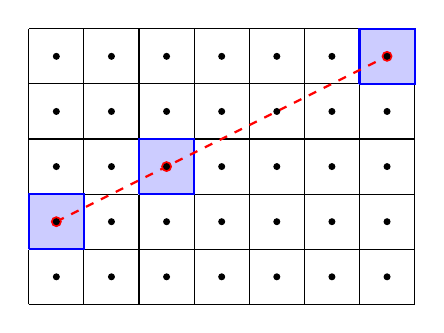
\begin{tikzpicture}[scale = 0.7]
    \draw[step=1.0,black,thin] (0,0) grid (7,5);
    \filldraw[blue!20!white] (0,1) rectangle (1,2);
    \filldraw[blue!20!white] (2,2) rectangle (3,3);
    \filldraw[blue!20!white] (6,4) rectangle (7,5);
    \draw[thick,blue] (0,1) -- (1,1) -- (1,2) -- (0,2) -- (0,1);
    \draw[thick,blue] (2,2) -- (2,3) -- (3,3) -- (3,2) -- (2,2);
    \draw[thick,blue] (6,4) -- (6,5) -- (7,5) -- (7,4) -- (6,4);
    \draw[dashed,red,thick] (0.5,1.5) -- (6.5,4.5);
    \filldraw[red] (0.5,1.5) circle (2.5pt);
    \filldraw[red] (2.5,2.5) circle (2.5pt);
    \filldraw[red] (6.5,4.5) circle (2.5pt);
    \foreach \X in {1,...,7}{
    \foreach \Y in {1,...,5}{
    \filldraw[black] (\X-0.5,\Y-0.5) circle (1.5pt);
    }
}
    
\end{tikzpicture}\\
\emph{An example of three squares with collinear centres}
\end{center}
